\documentclass[a4paper]{article}

%% Language and font encodings
\usepackage[spanish]{babel} % Adapta el documento al español (por ejemplo, cambia "Table of Contents" por "Índice") y gestiona la separación correcta de palabras al final de línea.
\usepackage[utf8]{inputenc} % Permite escribir directamente caracteres con tildes, la "ñ" o diéresis sin tener que usar comandos especiales.
\usepackage[T1]{fontenc} % Asegura que los caracteres acentuados se codifiquen correctamente en el archivo PDF final, permitiendo que se puedan copiar y pegar sin problemas.

%% Sets page size and margins
\usepackage[a4paper,top=3cm,bottom=2cm,left=3cm,right=3cm,marginparwidth=2cm]{geometry} % Define el tamaño de la página (A4) y los márgenes (superior, inferior, izquierdo y derecho).

%% Useful packages
\usepackage{amsmath,amsthm,amssymb} % Añade herramientas y comandos avanzados para escribir fórmulas y ecuaciones matemáticas complejas.
\usepackage{bm} % Escribir texto matemático en negrita
\usepackage{graphicx} % Permite insertar y manipular imágenes en el documento.
% \usepackage[colorinlistoftodos]{todonotes} % Facilita añadir notas o tareas pendientes ("TODOs") en los márgenes del documento mientras trabajas.
\usepackage[colorlinks=true, allcolors=blue]{hyperref} % Convierte las referencias, citas y el índice en enlaces clicables, y permite añadir enlaces a páginas web externas.
\usepackage{booktabs} % 

%% Definición del entorno para proposiciones
\theoremstyle{plain} % Estilo por defecto: título en negrita, cuerpo en cursiva
\newtheorem{prop}{Proposición}
%% Definición del entorno para corolarios
\theoremstyle{plain} % Estilo por defecto: título en negrita, cuerpo en cursiva
\newtheorem{corol}{Corolario}

%% Bibliography management
\usepackage{csquotes} % Proporciona comandos para manejar citas y comillas de manera consistente, especialmente útil cuando se trabaja con bibliografía y estilos de citación.
\usepackage[backend=biber, style=numeric]{biblatex} % Permite gestionar la bibliografía y las citas de manera avanzada, con soporte para diferentes estilos de citación. El backend "biber" se encarga de procesar la bibliografía.
\addbibresource{referencias.bib} 

\title{Un resolvedor codicioso totalmente automatizado para rompecabezas de piezas rectangulares irregulares y rotadas}
\author{José Manuel García Vergara, Jiahao Li, Fernanda Canales Martínez}

\begin{document}
\maketitle

\begin{abstract}
\noindent Este trabajo presenta el estudio, diseño, implementación y experimentación de un sistema totalmente automatizado para la resolución de rompecabezas digitales
(\textit{jigsaw puzzle solver}), tomando como fundamento teórico el modelo codicioso iterativo propuesto por Pomeranz, Sheffer y Truyen (CVPR 2011).
---TODO---

%% \noindent El resumen debe tener como máximo 250 palabras y ser un único párrafo. El resumen debe describir lo más fielmente posible el trabajo realizado (no el propuesto inicialmente, que podría ser distinto). 
%% En esta plantilla se presentan las indicaciones para realizar el trabajo de PID, al mismo tiempo que la estructura que debe tener la documentación a presentar. 

\hspace{1cm}

\noindent \textbf{Palabras clave:} 
%(hasta cinco palabras que clasifiquen el trabajo) 
PID, puzzle, solver, algoritmia, procesamiento de imágenes.
\end{abstract}


\section{Introducción}


---------

El trabajo de PID debe ser un trabajo de {\bf 50 horas por persona}, que sirva para profundizar en algunos aspectos del procesamiento de imágenes {\bf no vistos en clase}. Se debe trabajar sobre un tema concreto de procesamiento de imágenes {\bf apoyándose en artículo(s) de investigación} relativamente reciente(s) o en {\bf capítulos de libros científicos}.

El objetivo de los trabajos dirigidos consiste en explicar algún método o algoritmo de procesamiento de imágenes de una forma {\bf didáctica}, tanto teóricamente como de forma práctica. Es decir, 
\begin{itemize}
    \item primero, hay que {\bf estudiar el método teórico}, extrayendo las ideas principales de la documentación utilizada, comprendiendo todos los pasos y explicándolos de forma didáctica. Esto significa, por tanto, que {\bf no} debe hacerse una transcripción exacta de lo que aparece en el artículo de investigación referenciado.
    \item Segundo, hay que implementar o {\bf poner en práctica} el método, también de forma didáctica, tratando de mostrar pasos intermedios, significado de parámetros, experimentando, etc.
    \item Finalmente hay que hacer una {\bf presentación didáctica} del método,  explicando cada uno de los pasos requeridos para llegar al resultado final.

\end{itemize}

Los trabajos se realizarán en grupos de trabajo preferiblemente de {\bf tres} personas.  A partir de la explicación de las instrucciones del trabajo en grupo, las clases indicadas en el {\bf Calendario} se dedicarán a la realización del trabajo y seguimiento, por parte del profesorado, del trabajo del grupo. 

Se recomienda usar alguna herramienta de planificación y gestión de proyectos para hacer una planificación inicial y un seguimiento posterior del desarrollo del trabajo, registrando las tareas realizadas por cada uno (y el tiempo empleado). Téngase en cuenta que las horas de dedicación de \textbf{cada alumno/a} han de ser \textbf{50 horas}. Será obligatorio presentar los tiempos realizados {\bf individualmente en cada sesión de seguimiento.}

\section{Planteamiento teórico}

\subsection{Representación del espacio de color y extracción de características}
\label{representaciondelespaciodecoloryextracciondecaracteristicas}

La elección del espacio de color es determinante para modelar la compatibilidad visual entre los píxeles de la imagen. 
Aunque se capturan comúnmente en el espacio RGB, este carece de uniformidad perceptiva: una distancia euclídea en RGB no se corresponde
con la diferencia cromática percibida por el sistema visual humano.

Por esta razón, el sistema realiza una conversión al espacio de color \textit{CIE LAB}, donde el canal \textit{L} codifica la luminancia perceptiva 
y los canales \textit{A} y \textit{B} representan las dimensiones cromáticas oponentes (verde-rojo y azul-amarillo, respectivamente). Esta descomposición
desacopla la información de brillo de las variaciones cromáticas, permitiendo que la métrica de compatibilidad opere en una representación perceptual linealizada.

A diferencia del paper de referencia \cite{articulopomeranz}, en este proyecto no se hace uso de un espacio \textit{CIE LAB normalizado} ya que 
no resulta útil (véase \ref{expEspaciosColor} y \ref{invarianteCompatibilidad}).


\subsection{Métrica de disimilitud de bordes predictiva}

\subsection{Conversión a compatibilidad mediante normalizadión adaptativa por cuartil}

\subsection{Relaciones de máxima confianza recíproca: Best Buddies}

\subsection{El colocador voraz: The Placer}

\subsection{Extracción de componentes conexas y refinamiento iterativo: Segmenter y Shifter}





-----

La sección \textit{Planteamiento teórico} debe plantear el problema a resolver, así como describir los algoritmos propuestos para su resolución. 

La realización del trabajo está programada en {\bf 3 fases}, en cada una de las cuales se realiza un {\bf Seguimiento} que consiste en que todos los miembros del grupo le explican sus progresos a la profesora y cada miembro entrega un pequeño informe individual del trabajo realizado hasta el momento. {\bf Estos seguimientos son obligatorios}. Se debe hablar con la profesora en caso de dificultades para asistir. Al final de los seguimientos, la profesora asignará un {\bf coeficiente corrector (entre 0 y 1) individual a la nota de trabajo conjunta, en base al trabajo individual realizado por cada mienmbro del grupo. }
\subsection*{FASE 1}
En la primera fase, \textbf{los miembros del grupo} realizarán la \textbf{propuesta del trabajo dirigido} (TD), acordando con el profesorado el trabajo a realizar. 

Para la búsqueda de libros y bases de datos de revistas, se puede consultar el catálogo fama de la US \url{http://fama.us.es/}. Se recomiendan las bases de datos ScienceDirect (Elsevier), IEEE Xplore y Sringerlink. Si se accede desde fuera de la Universidad, se tendrá que usar el UVUS. Se pueden encontrar recursos para buscar ideas en el documento \textit{Enlaces de interés} del contenido en ev.

En la \textbf{Fase 1}, se debe entregar la {\bf planificación inicial} y la {\bf lista de objetivos} del TD. En la planificación se debe describir cómo se distribuirán las {\bf 50 horas/persona} que el grupo debe dedicar al TD, incluidas las sesiones de clase dedicadas al trabajo.  
En esta fase debe comprenderse la teoría relativa al trabajo a realizar y quedar perfectamente definido. 

\subsection*{FASE 2}
En esta fase se comenzará a trabajar en la parte práctica y explicación del método. Se recomienda comenzar a escribir la documentación desde el principio.

El algoritmo (o algoritmos) a implementar debe estar perfectamente claro y diseñado. Al finalizar la Fase 2, se mostrará una primera versión de la implementación, algo mínimo. Se puede hacer "fork" de un repositorio ya existente, {\bf dejando claro la contribución/adaptación/ experimentación propia}. Toda la implementación debe organizarse en un repositorio que se compartirá con la profesora.

Se procurará tener un producto mínimo viable de la implementación al final de la fase, así como una primera versión de la documentación. 

 Se mostrará la hoja de tiempos realizada hasta ese momento y \textbf{se revisarán los objetivos iniciales} planteados.

\subsection*{FASE 3}

En la última fase se realizará la experimentación para poder evaluar y comparar el método implementado y poder inferir conclusiones. Al final de la Fase 3, se tendrá una primera versión de la presentación (aunque sólo sea un índice), junto con una revisión de la documentación y de la implementación. 

\vspace{1cm}
En la siguiente tabla se resumen los hitos que deben alcanzarse (y entregarse) al final de cada Fase: 

    \begin{center}
    \begin{tabular}{|c||l|}
    \hline
  Seguimiento 1 & Propuesta del TD basándose en una fuente científica.   \\& Planificación inicial y lista de objetivos. \\
  & Estudio y comprensión del método elegido. \\
  & Hoja de tiempos individual.\\
\hline
Seguimiento 2  & Primera versión de la implementación y de la documentación. \\ &  Hoja de tiempos individual.\\& Revisión de los objetivos. \\
\hline
 Seguimiento 3  & Primera versión de la presentación.  \\& Revisión de la documentación  y de la  implementación.\\&  Hoja de tiempos individual.\\
\hline
    \end{tabular}
    \end{center}
Los días dedicados a Seguimiento aparecen en el Calendario publicado en ev. Cada grupo tendrá que agendar con la profesora al menos 3 reuniones para los seguimientos obligatorios.

\textbf{Todos} los miembros del grupo deberán \textbf{intervenir en la exposición final}, en la que deberán defender su trabajo y comentar los logros teóricos y de implementación obtenidos. Además, deberá hacerse algún ejemplo usando la implementación desarrollada (\textbf{20 minutos en total}). Las exposiciones se realizarán en horario de clase en las dos últimas semanas. Después se abrirá un turno de preguntas.

Para la entrega, cada grupo deberá subir, en respuesta a una actividad creada para tal efecto en la ev, los siguientes elementos:

 \begin{itemize}
\item \url{documentacion.pdf}. Consiste en un fichero \url{.pdf} correspondiente a la documentación. 

Estructura de la documentación:

\begin{enumerate}
\item[]  Título
\item[]  Autores
\item[]  Resumen
\item  Introducción 
\item  Planteamiento teórico 
\item  Implementación
\item  Experimentación
\item  (Manual de usuario)
\item Uso de IA en este trabajo
\item  Conclusiones
\item Autoevaluación de cada miembro
\item  Tabla de tiempos
\item[]  Bibliografía
\end{enumerate}

Se puede usar el fichero \url{main.tex} disponible en enseñanza virtual como plantilla de Latex\footnote{Véase el Anexo para algunos apuntes rápidos sobre escritura de textos en LaTex (tomados de \url{Overleaf.com}.}, que es el que se ha usado en este documento. Se recomienda el uso de editores online de LaTeX como \url{Overleaf.com}, aunque a día de hoy, la versión gratuita sólo permite dos colaboradores.

Las referencias se citan así:
bla, bla \cite{articulopomeranz}, bla, bla \cite{nuestrorepo}. La bibliografía
debe seguir el estilo de este documento, con las referencias ordenadas alfabéticamente por autores.

También se puede documentar el trabajo en un Notebook de Jupyter, en el que también se puede incluir código LaTex e imprimirlo como pdf.

\item \url{Repositorio}. Se debe crear un repositorio github, y referenciarlo en la documentación. 

Si se ha desarrollado una aplicación propia, debe contener todo el código utilizado, comentado y modulado. Debe contener el ejecutable, si existiera, junto con todos los archivos necesarios para su ejecución de forma que no dé errores de compilación.
Debe contener un {\bf Readme} con instrucciones para ejecutar el código.
Se debe incluir una carpeta \textbf{images} con imágenes de muestra, incluyendo las imágenes usadas en la experimentación.

En caso de que exista ya una implementación en un repositorio público asociado al trabajo escogido, se debe desarrollar una versión propia, haciendo una bifurcación (fork) del repositorio que incluya explicaciones, paso a paso, ejemplos, modificaciones, etc. Por ejemplo, se puede hacer un notebook de jupyter que incluya ejemplos de uso o la experimentación.
Aquí el archivo {\bf Readme} deberá referenciar bien el trabajo original y explicar la aportación propia.


\item \url{presentacion.pdf}. Consiste en un fichero \url{.pdf} con la presentación que se usará en clase para exponer el trabajo.
\end{itemize}

La evaluación del trabajo se realizará en base a una rúbrica que se proporcionará en la ev. 




\section{Implementación}

Esta sección de la documentación  debe incluir la descripción de la implementación (pero no el código), especificando las tecnologías usadas, el diseño, módulos o partes principales. \textbf{Debe quedar muy claro cuál es la parte original implementada, qué repositorio se ha adaptado o bifurcado, qué librerías se han usado,  todo con referencias apropiadas}. Se debe describir (tanto en la aplicación, como en la documentación, como en la presentación) los pasos seguidos para resolver el problema que se plantea de la forma más divulgativa posible. 

%Se recomienda el uso de Python con la librería \textbf{OpenCV}, \url{https://opencv.org/}.
%Matlab posee también un toolbox de procesamiento de imágenes que se puede usar en los laboratorios de la escuela.
Una opción muy práctica y recomendable es la de usar la librería \textbf{OpenCV} con Python mediante el gestor de paquetes de Anaconda \url{https://www.anaconda.com} y usar los notebook de Jupyter en los que se puede intercalar ejecución de código con explicaciones teóricas. % Éstas sólo son algunas indicaciones. 

Siempre se debe redactar un fichero {\bf Leeme explicando todo lo necesario para poder ejecutar y usar la implementación} en cualquier ordenador (o al menos con el mismo sistema operativo).



\section{Experimentación}
\subsection{Espacios de color, normalización y ratios discriminativos}
\label{expEspaciosColor}
En primer lugar, evaluamos empíricamente sobre el puzzle de Lisboa de 150 piezas la capacidad del sistema bajo cuatro modalidades de preprocesamiento en el espacio LAB:

\begin{itemize}
    \item \textbf{Método 1 (Actual - OpenCV uint8):} Representación nativa con $L, A, B \in [0, 255]$.
    \item \textbf{Método 2 (Escalado uniforme $\bm{[0, 1]}$):} Método 1 dividido por $255$.
    \item \textbf{Método 3 (CIELAB Estándar):} Conversión en coma flotante con $L \in [0, 100]$ y $A, B \in [-127, 127]$.
    \item \textbf{Método 4 (CIELAB Normalizado por canal):} $L/100$, $(A + 127)/254$, $(B + 127)/254$.
\end{itemize}

Para medir la capacidad de discriminación, definimos el \textit{Ratio Discriminativo} como el cociente entre la compatibilidad media de los pares vecinos reales del Ground Truth y la compatibilidad media con los candidatos falsos:

\begin{equation*}
    R_{\text{disc}} = \frac{\mathbb{E}[C(\text{vecinos reales})]}{\mathbb{E}[C(\text{vecinos espurios})]}
\end{equation*}


\textbf{Análisis de resultados:} Como se observa en el Cuadro \ref{tab:comparativa_lab}, el Método 1 y el Método 2 ofrecen resultados exactamente equivalentes (discrepancia numérica máxima de $6'17 \times 10^{-7}$, 
producto del redondeo de coma flotante). A raíz de este dato, surgió la hipótesis de invarianza de escala que se demuestra matemáticamente en el apéndice \ref{invarianteCompatibilidad}. Además, la representación nativa de OpenCV proporciona una 
relación señal-ruido superior ($R_{\text{disc}} = 1'2219$), superando a las variantes estandarizadas.

\begin{table}[htbp]
\centering
\caption{Comparativa de representaciones en el espacio LAB (Lisboa $10 \times 15$, 150 piezas cuadradas, 550 bordes dirigidos).}
\label{tab:comparativa_lab}
\begin{tabular}{lcccc}
\toprule
\textbf{Método de representación} & \textbf{Top-1 (\%)} & \textbf{Aciertos} & \textbf{Precisión BB (\%)} & \textbf{Ratio $R_{\text{disc}}$} \\
\midrule
Método 1 (OpenCV nativo uint8) & \textbf{99.64\%} & \textbf{548/550} & \textbf{99.64\% (546/548)} & \textbf{1.2219} \\
Método 2 (Escalado uniforme $[0,1]$) & \textbf{99.64\%} & \textbf{548/550} & \textbf{99.64\% (546/548)} & \textbf{1.2219} \\
Método 3 (CIELAB estándar float) & 99.45\% & 547/550 & 99.45\% (545/548) & 1.2042 \\
Método 4 (Normalizado por canal) & 99.27\% & 546/550 & 99.27\% (544/548) & 1.2013 \\
\bottomrule
\end{tabular}
\end{table}

\section{Manual de usuario}

Se debe incluir un breve manual de usuario en caso de que se desarrolle una aplicación propia. Si se implementa un notebook de Jupyter, no es necesario un manual de usuario, sino que debe quedar muy guiado, explicando todos los pasos y parámetros.  

\section{Uso de IA en este trabajo} Se pueden utilizar herramientas de IA en cualquier fase y con cualquier alcance. Su uso no está limitado, pero debéis \textbf{declararlo con claridad y ser capaces de explicar y defender las decisiones, la teoría, el código y los resultados del trabajo.} 

Se deben incluir los siguientes puntos:

\begin{itemize}
    \item \textbf{Herramientas usadas:} servicio, modelo o agente concreto, forma de acceso y tipo de cuenta (personal o proporcionada por la universidad; gratuita o de pago).
    \item \textbf{Objetivo:} aprendizaje de la teoría, búsqueda de fuentes, elección del método, desarrollo o depuración del código, datos y experimentos, análisis de resultados, figuras y documentación. Se deben señalar los archivos o apartados afectados. Si se partió de un repositorio, hay que citarlo y distinguir su contenido de las aportaciones propias y de las realizadas con ayuda de IA.
    \item \textbf{Verificación de las respuestas:} las respuestas dadas por una herramienta IA, no deben tomarse como verdades absolutas. Las consultas deben hacerse solicitando que la respuesta se fundamente en fuentes fiables o realizar comprobaciones sobre las respuestas obtenidas. Se deben aportar fuentes consultadas, pruebas del código, revisión de las imágenes y comprobación de los resultados. Se debe mencionar cualquier error relevante que se detecte y corrija.
    \item \textbf{Datos y permisos}: declaración de imágenes, datos personales, material de terceros, código del repositorio o partes del trabajo que se introdujeron en la IA y bajo qué permiso o licencia se utilizaron. Identificación  del material sintético o modificado con IA que forme parte de la entrega.
    \item \textbf{Trazabilidad:} Incluir dos o tres ejemplos representativos de instrucciones dadas a la IA, resumiendo qué respuesta se aprovechó, qué se cambió o descartó. Si el uso fue amplio, añadid un registro breve en un anexo o en el repositorio, sin necesidad de entregar el historial completo de conversaciones.
\end{itemize}


 En la defensa, cualquier integrante del grupo deberá poder explicar las partes esenciales del trabajo, con independencia de cómo se hayan desarrollado.

\section{Conclusiones}

Se debe introducir una sección de conclusiones que incluyan propuestas claras de mejora o extensión del trabajo (por ejemplo, si no se han podido alcanzar todos los objetivos iniciales). También conclusiones sobre los resultados obtenidos, en qué medida difieren de los esperados. Además, son apropiadas conclusiones sobre las desviaciones en cuanto a la planificación inicial de tiempos, así como conclusiones sobre la experiencia de la realización del trabajo (lecciones aprendidas) y sobre el uso de IA en su elaboración.

\section{Autoevaluación}

Siguiendo la rúbrica dada, se debe detallar, por parte de  \textbf{cada miembro del grupo}, la puntuación para el trabajo que se considera justa en cada apartado. 

\section{Tabla de tiempos}


Se debe justificar el trabajo realizado por cada componente del grupo, indicando el {\bf tiempo total que cada miembro del grupo ha dedicado} al trabajo (lo que puede implicar diferencia de notas obtenidas por los distintos miembros del grupo). El trabajo realizado debe ser de {\bf 50 horas por estudiante}. Además, debe haber un plan de trabajo \textbf{individual} detallado con las {\bf tareas específicas realizadas por cada miembro} del grupo. Ejemplos de tareas son: implementación de la función "tal" del código; búsqueda de información y redacción del concepto "tal"; Generación de tabla ilustrativa para el proceso "tal". No son tareas: escribir la documentación; desarrollar código; hacer la presentación. Se puede usar la tabla siguiente o bien documentos generados por la herramienta de gestión de proyectos que se prefiera.

\begin{center}
\begin{tabular}{|c|c|c|c|}
\hline
 Fecha de la
 actividad 
& Tiempo (h)
& Miembro
& Actividad realizada
\\\hline
\mbox{ }&\mbox{}&\mbox{ }&\mbox{}\\
\mbox{ }&\mbox{}&\mbox{ }&\mbox{}\\\hline
\end{tabular}
\end{center}

\nocite{*}
\printbibliography[title={Referencias}]

Ejemplo de citación \cite{articulopomeranz} y referencias \cite{nuestrorepo}.


\section{Apéndice}
\subsection{¿Por qué la compatibilidad es invariante ante un escalado uniforme?}
\label{invarianteCompatibilidad}

Se va a usar el planteamiento teórico de Pomeranz, por mayor simplicidad. 
No obstante, las conclusiones obtenidas son directamente generalizables a la métrica
extendida propuesta en este trabajo.

\begin{prop} [Invarianza de Escala]
Sea $\alpha \in \mathbb{R}^+$ un factor de escala estrictamente positivo aplicado uniformemente sobre todos los canales y píxeles de las piezas del puzzle, tal que $x'_i = \alpha x_i$ para todo $i \in \{1, ..., N\}$. Entonces, la matriz de compatibilidad resultante $C'$ es idéntica a la matriz original $C$:
$$C'(x_i, x_j, R) = C(x_i, x_j, R) \quad \forall i, j \in \{1, ..., N\}, \forall R \in \{\text{arriba}, \text{abajo}, \text{izquierda}, \text{derecha}\}$$
\end{prop}
\begin{proof}   
% \textbf{Paso 1: Escalado de los descriptores de frontera y la predicción}

Al aplicar la transformación lineal $x'_i = \alpha x_i$, los vectores de frontera heredan directamente el factor de escala:
$$B_1(x'_i, R) = \alpha B_1(x_i, R), \quad B_2(x'_i, R) = \alpha B_2(x_i, R)$$
donde $B_1(x_i,R),B_2(x_i,R) \in \mathbb{R}^{K \times 3}$ son los píxeles de la frontera exterior misma de la pieza (la última línea de píxeles adyacentes a la pieza vecina) y
los píxeles de la frontera interior contigua (la penúltima línea de píxeles), respectivamente.

Por linealidad del operador de diferencias finitas, el vector de predicción de Taylor escala homogéneamente:
\begin{align*}
\text{Pred}(x'_i, R) &= 2B_1(x'_i, R) - B_2(x'_i, R) = 2(\alpha B_1(x_i, R)) - \alpha B_2(x_i, R) = \alpha(2B_1(x_i, R) - B_2(x_i, R)) \\
&= \alpha \text{Pred}(x_i, R)
\end{align*}

% \textbf{Paso 2: Homogeneidad del término de error fraccionario}

Evaluando la diferencia absoluta entre la predicción escalada y el borde exterior del candidato vecino:
\begin{align*}
|\text{Pred}(x'_i, R)_{k,c} - B_1(x'_j, R_{op})_{k,c}|^p &= |\alpha \text{Pred}(x_i, R)_{k,c} - \alpha B_1(x_j, R_{op})_{k,c}|^p \\
&= |\alpha (\text{Pred}(x_i, R)_{k,c} - B_1(x_j, R_{op})_{k,c})|^p    
\end{align*}
donde $R_{op}$ es la dirección opuesta a $R$.


Dado que $\alpha > 0$, aplicando la propiedad multiplicativa del valor absoluto $|a \cdot b| = |a| \cdot |b|$:
$$|\alpha (\text{Pred}(x_i, R)_{k,c} - B_1(x_j, R_{op})_{k,c})|^p = \alpha^p |\text{Pred}(x_i, R)_{k,c} - B_1(x_j, R_{op})_{k,c}|^p$$

El mismo desarrollo aplica de manera idéntica al término simétrico inverso de $x_j$ hacia $x_i$.

% \textbf{Paso 3: Factorización de la disimilitud}

Sustituyendo ambos términos escalados en la ecuación de disimilitud:
$$D'(x_i, x_j, R) = \left[ \sum_{k=1}^{K} \sum_{c=1}^{3} \left( \alpha^p |\text{Pred}(x_i, R)_{k,c} - B_1(x_j, R_{op})_{k,c}|^p + \alpha^p |\text{Pred}(x_j, R_{op})_{k,c} - B_1(x_i, R)_{k,c}|^p \right) \right]^{\frac{1}{p}}$$

Extrayendo $\alpha^p$ como factor común del doble sumatorio:
$$D'(x_i, x_j, R) = \left[ \alpha^p \sum_{k=1}^{K} \sum_{c=1}^{3} \left( |\text{Pred}(x_i, R)_{k,c} - B_1(x_j, R_{op})_{k,c}|^p + |\text{Pred}(x_j, R_{op})_{k,c} - B_1(x_i, R)_{k,c}|^p \right) \right]^{\frac{1}{p}}$$

Aplicando la propiedad de las potencias $(u \cdot v)^\gamma = u^\gamma \cdot v^\gamma$ con $\gamma = 1/p$:
$$D'(x_i, x_j, R) = (\alpha^p)^{\frac{1}{p}} \cdot \left[ \sum_{k=1}^{K} \sum_{c=1}^{3} (...) \right]^{\frac{1}{p}} = \alpha \cdot D(x_i, x_j, R)$$

Es decir, toda la matriz de disimilitud queda uniformemente escalada por la constante global $\alpha$.

% \textbf{Paso 4: Propiedad de escala en estadísticos de orden (cuartil)}

Sea $S_i = \{D(x_i, x_m, R) \mid m \neq i\}$ el conjunto de disimilitudes de la fila $i$. Al escalar todos sus elementos por la constante positiva $\alpha$, el conjunto transformado es $S'_i = \{\alpha \cdot d \mid d \in S_i\}$. Dado que la multiplicación por un escalar positivo es monótona creciente, preserva estrictamente el orden de los elementos. Por consiguiente, cualquier cuantil de orden $\tau \in [0, 1]$ cumple:
$$Q_\tau(S'_i) = \alpha \cdot Q_\tau(S_i)$$

En particular, para el primer cuartil ($\tau = 0.25$):
$$\text{quartile}'(i, R) = \alpha \cdot \text{quartile}(i, R)$$

% \textbf{Paso 5: Cancelación algebraica en el exponente de compatibilidad}

Sustituyendo $D'$ y $\text{quartile}'$ en la formulación de compatibilidad:
$$C'(x_i, x_j, R) = \exp\left( -\frac{D'(x_i, x_j, R)}{\text{quartile}'(i, R)} \right) = \exp\left( -\frac{\alpha \cdot D(x_i, x_j, R)}{\alpha \cdot \text{quartile}(i, R)} \right)$$

Cancelando el factor común $\alpha \neq 0$ en el cociente del exponente:
$$C'(x_i, x_j, R) = \exp\left( -\frac{D(x_i, x_j, R)}{\text{quartile}(i, R)} \right) = C(x_i, x_j, R)$$

Quedando demostrada la proposición.     
\end{proof}

\begin{corol}
Como consecuencia directa de este resultado, cualquier reescalado homogéneo de la representación de color (como mapear el rango discreto de intensidades estándar de OpenCV 
$[0,255]$ al intervalo continuo $[0,1]$ mediante $\alpha = 1/255$) produce exactamente las mismas matrices de compatibilidad 
$C$, preservando de forma idéntica los órdenes de clasificación (rankings), los máximos por fila (argmax) 
y, por consiguiente, la totalidad de las relaciones recíprocas de Best Buddies.
\end{corol}




\end{document}


























%% COSAS ANTERIORES ------------------------------------------------------------------------------------------------------------------------

\begin{thebibliography}{10}



\bibitem{clave:libro}
U. N. Experto, \emph{Un libro que escribí},
Editorial, 1996.

\bibitem{clave:revista}
Y. O. Mismo,
``Título del artículo'',
\emph{Revista Publicación Periódica}, Vol. 17, pp. 1-100, 1997.
\end{thebibliography}

\newpage 

\section*{More about how to write an article}
\subsection{How to include Figures}

First you have to upload the image file from your computer using the upload link the project menu. Then use the includegraphics command to include it in your document. Use the figure environment and the caption command to add a number and a caption to your figure. See the code for Figure \ref{fig:frog} in this section for an example.

\begin{figure}[h]
\centering
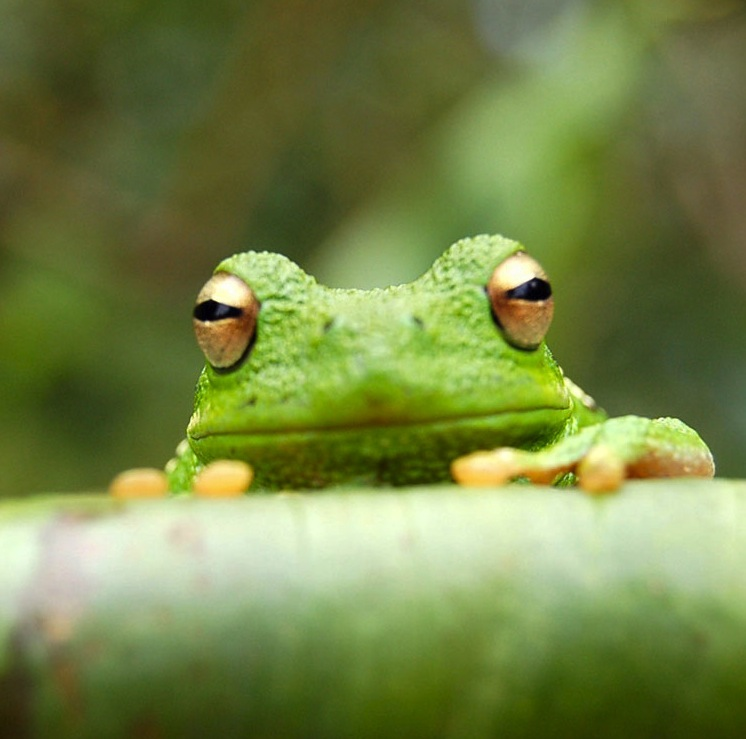
\includegraphics[width=0.3\textwidth]{frog.jpg}
\caption{\label{fig:frog}This frog was uploaded via the project menu.}
\end{figure}


\subsection{How to add Tables}

Use the table and tabular commands for basic tables. See Table~\ref{tab:widgets}, for example. 

\begin{table}[h]
\centering
\begin{tabular}{l|r}
Item & Quantity \\\hline
Widgets & 42 \\
Gadgets & 13
\end{tabular}
\caption{\label{tab:widgets}An example table.}
\end{table}

\subsection{How to write Mathematics}

\LaTeX{} is great at typesetting mathematics. Let $X_1, X_2, \ldots, X_n$ be a sequence of independent and identically distributed random variables with $\text{E}[X_i] = \mu$ and $\text{Var}[X_i] = \sigma^2 < \infty$, and let
\[S_n = \frac{X_1 + X_2 + \cdots + X_n}{n}
      = \frac{1}{n}\sum_{i}^{n} X_i\]
denote their mean. Then as $n$ approaches infinity, the random variables $\sqrt{n}(S_n - \mu)$ converge in distribution to a normal $\mathcal{N}(0, \sigma^2)$.


\subsection{How to create Sections and Subsections}

Use section and subsections to organize your document. Simply use the section and subsection buttons in the toolbar to create them, and we'll handle all the formatting and numbering automatically.

\subsection{How to add Lists}

You can make lists with automatic numbering  or bullet points \dots

\begin{enumerate}
\item Like this,
\item and like this.
\end{enumerate}

\begin{itemize}
\item Like this,
\item and like this.
\end{itemize}

%\subsection{How to add Citations and a References List}

%You can upload a \verb|.bib| file containing your BibTeX entries, created with JabRef; or import your \href{https://www.overleaf.com/blog/184}{Mendeley}, CiteULike or Zotero library as a \verb|.bib| file. You can then cite entries from it, like this: \cite{greenwade93}. Just remember to specify a bibliography style, as well as the filename of the \verb|.bib|.

%You can find a \href{https://www.overleaf.com/help/97-how-to-include-a-bibliography-using-bibtex}{video tutorial here} to learn more about BibTeX.



%\bibliographystyle{alpha}
%\bibliography{sample}

\end{document}